\documentclass[11pt]{article}

\usepackage[margin=1in]{geometry}
\usepackage{amsmath,amssymb}
\usepackage{booktabs}
\usepackage{hyperref}
\usepackage{xcolor}
\usepackage{parskip}
\usepackage{fancyhdr}
\usepackage{graphicx}

\pagestyle{fancy}
\fancyhf{}
\fancyhead[C]{\small\color{red!70!black}\bfseries INTERNAL WORKING DRAFT --- NOT FOR CIRCULATION --- NOTHING HERE IS ARXIV-READY}
\renewcommand{\headrulewidth}{0.4pt}

\title{Accretion-Modified Dynamical Friction and Stone Skipping\\ of Black Holes in Ultralight Dark Matter\\[4pt]
\large (Working Title --- Taproot Draft)}
\author{}
\date{Draft status as of \today}

\newcommand{\code}[1]{\texttt{#1}}
\newcommand{\TODO}[1]{\textcolor{red}{\textbf{[TODO: #1]}}}
\newcommand{\OPEN}[1]{\textcolor{orange!80!black}{\textbf{[OPEN: #1]}}}

\begin{document}
\maketitle

\begin{center}
\fbox{\begin{minipage}{0.9\textwidth}
\small
\textbf{Status note.} This document exists to establish scope and structure before any
writing that could end up in a paper. Nothing in it is checked to submission
standard. Every quantitative claim below is either (a) directly reproducible
from a script/run in this repository, tagged as such, or (b) marked
\OPEN{...} / \TODO{...} as not yet done. Treat this as a lab notebook that
happens to be typeset, not a manuscript draft.
\end{minipage}}
\end{center}

\tableofcontents

\section{Research questions}

Two prior, independent results treat the black hole (or test-mass perturber)
as having \emph{fixed mass} throughout the simulation:

\begin{enumerate}
  \item \textbf{Dynamical friction in a uniform ULDM background.} Lancaster,
    Giovanetti, Mocz, Kahn, Lisanti \& Spergel (2019), arXiv:1909.06381, is
    the foundational analytic + numerical treatment. Wang \& Easther (2021),
    arXiv:2110.03428, extends this to a point mass in a uniform background
    and then an SMBH embedded in a soliton, establishing baseline friction
    timescales.
  \item \textbf{Stone skipping in a soliton.} Zhang, Wang, Zagorac \&
    Easther (2026), arXiv:2602.11512, shows that a black hole orbiting
    inside a soliton can undergo non-monotonic, quasi-periodic radial
    excursions (``stone skipping''), driven by a dipole resonance between
    the orbit and a soliton oscillation mode, modelled as a forced damped
    harmonic oscillator.
\end{enumerate}

\textbf{The proposed new work}: repeat both scenarios with the black hole's
mass allowed to \emph{grow via accretion} of the surrounding ULDM, using the
sink mechanism already implemented in this codebase
(\code{PyUltraLight2.Particles.Accretion}), and ask whether/how mass growth
modifies each phenomenon:

\begin{itemize}
  \item \textbf{Modified dynamical friction}: does a growing $M(t)$
    accelerate or otherwise qualitatively change the inspiral, given that
    dynamical friction forces scale $\propto M^2$ in the classical
    (Chandrasekhar-type) treatment? Is there a runaway/self-reinforcing
    regime?
  \item \textbf{Modified stone skipping}: does mass growth detune the
    dipole resonance (since the resonance condition is mass-ratio
    dependent), damp the oscillation, or alter its period/amplitude over
    the run?
\end{itemize}

\OPEN{These are two separate simulation campaigns (uniform background vs.
soliton), not one. Neither has been started yet beyond the accretion
machinery validation below.}

\OPEN{Unresolved wrinkle for the dynamical-friction campaign specifically:
this project's own unpublished exploration (uniform background + full
self-gravity, \emph{no} accretion) already found runaway gravitational
collapse rather than steady dynamical friction — a qualitatively different
baseline behaviour from Lancaster et al.'s regime. Needs to be understood/
reconciled (transient-wave-structure regime where their analytics break
down? parameter choice?) before accretion is layered on top, or the
``modified dynamical friction'' framing may need to lead with a different
baseline.}

\section{Physical setup (as implemented)}

Ultralight/fuzzy dark matter obeys the Schr\"odinger--Poisson system
\begin{align}
  i\hbar\,\partial_t \psi &= \left[-\frac{\hbar^2}{2m}\nabla^2 + m\Phi\right]\psi, &
  \nabla^2\Phi &= 4\pi Gm|\psi|^2,
\end{align}
evolved pseudospectrally (operator-split kick--drift--kick, FFT Poisson
solve) on a periodic grid. A classical point-mass black hole is coupled
two-way: it feels $\Phi$ (interpolated, RK4-integrated motion) and sources a
Plummer-softened potential $\Phi_{TM}(r) = -am/\sqrt{1+a^2r^2}$ added to the
field.

Accretion is added as a local imaginary potential (a moving sink):
\begin{equation}
  \psi \mathrel{*}= \exp\!\big[-h\,V_{\rm sink}(\mathbf r,t)\big], \qquad
  V_{\rm sink}(\mathbf r) = A\exp\!\left(-\frac{|\mathbf r-\mathbf r_{\rm BH}|^2}{2R^2}\right),
\end{equation}
with the removed mass $\Delta M = V_{\rm cell}\sum(\rho_{\rm before}-\rho_{\rm after})$
added to the black hole, and (optionally) the removed momentum
$\int \mathbf j(\mathbf r)(1-e^{-2hV_{\rm sink}})\,dV$, with
$\mathbf j = \mathrm{Im}(\psi^*\nabla\psi)$, deposited onto its velocity as
a rocket-equation update (drag/recoil from the swallowed matter). $A,R$ can
be fixed, or dynamically recalibrated every step from the particle's
instantaneous mass and speed to track the classical Bondi--Hoyle--Lyttleton
rate,
\begin{equation}
  \dot M_{\rm BHL} = \frac{4\pi(GM)^2\rho}{(v_{\rm rel}^2+c_s^2)^{3/2}}
  \quad\Rightarrow\quad
  R = \frac{2M}{v_{\rm rel}^2+c_s^2}, \qquad
  A = \frac{(v_{\rm rel}^2+c_s^2)^{3/2}}{8\sqrt{2\pi}\,M}.
\end{equation}
$v_{\rm rel}$ is the black hole's velocity relative to the \emph{local} ULDM
flow (interpolated current $\mathbf j/\rho$ at the particle's position), not
its raw box-frame speed — see \S\ref{sec:validation} for why that distinction
turned out to matter. Full API in \code{UserManual.tex} (this repository).

\section{Related work and positioning}
\label{sec:related}

\textbf{Fixed-mass dynamics baselines} (\S\ref{}, item list above):
Lancaster et al. 2019 (1909.06381); Wang \& Easther 2021 (2110.03428);
Zhang, Wang, Zagorac \& Easther 2026 (2602.11512, ``stone skipping'').

\textbf{Accretion literature} — checked directly (live search, not
memorised) 2026-09-29, since a first pass at this framing risked an
inaccurate ``nobody has looked at BH+FDM accretion'' claim:

\begin{itemize}
  \item Cardoso, Ikeda, Vicente \& Zilh\~ao (2022), PRD Letters,
    arXiv:2207.09469, ``Parasitic black holes'' — full numerical relativity,
    spherically symmetric, a \emph{static} BH swallowing a boson star.
    Different regime (GR near-horizon, no moving particle, no BHL rate).
    Low direct methodological overlap, but closest-sounding title —
    must cite to preempt ``have you seen this?''.
  \item Chiu, Schive, Yang, Huang \& Gaspari (2025), PRL, arXiv:2501.09098
    — \emph{static} soliton potential boosting Bondi accretion of a
    \textbf{separate baryonic gas component}; the FDM field itself is never
    absorbed.
  \item Ludwig, Mocz \& Robles (2026), PRD, arXiv:2607.00349 (submitted
    Jul 2026) — \textbf{closest prior work}. Live, moving BH in a live
    Schr\"odinger--Poisson soliton, explicitly benchmarked against
    $\dot M_{\rm BHL}$. Sink removes mass from a \textbf{separate isothermal
    gas mesh} (FLASH-style cloud-in-cell deposition, strictly
    mass-conserving), not the ULDM wavefunction; sink radius \textbf{fixed}
    at $2.5\Delta x$ (grid-tied); BHL used only as an external diagnostic
    target, never fed back into the sink's own geometry.
\end{itemize}

\textbf{Defensible novelty niche} (not ``first to study this''): (a) direct
non-Hermitian absorption of the dark matter field itself, not a gas proxy;
(b) sink geometry dynamically slaved to BHL every step from instantaneous
$(M,v_{\rm rel})$, not fixed-radius-with-external-diagnostic; (c) explicit
momentum/recoil deposition from the absorbed field's local current, not a
pure mass leak. \TODO{Related-work section of any actual manuscript must
explicitly position against Ludwig et al. 2607.00349 — omitting it reads as
either unaware of very recent literature or dodging it.}

\section{Validation status of the accretion machinery}
\label{sec:validation}

Everything in this section is directly reproducible from this repository
(see \code{CHANGES.md} for the dated, itemised history; \code{Analysis/}
for the checking scripts).

\begin{itemize}
  \item \textbf{Mass conservation}: exact to $\sim 10^{-12}$ relative
    (grid mass lost = sink mass gained), checked at every resolution tried
    so far (32--64, \S\ref{sec:convergence}).
  \item \textbf{Momentum conservation}: direct check via
    $\int\mathrm{Im}(\psi^*\nabla\psi)\,dV + M\mathbf v$ at $48^3$. Gravity-only
    baseline has residual drift $\sim10^{-3}$ (grid/interpolation noise
    floor). Sink \emph{without} momentum deposit: drift $-0.35$
    ($\sim310\times$ the floor — the mass-leak-with-no-recoil problem was
    real). Sink \emph{with} it: drift $+0.0055$ ($\sim5\times$ the floor,
    $64\times$ improvement). \OPEN{Residual not at machine precision; not
    yet root-caused (candidates: finite-$h$ discretisation, or consistent
    with the same noise floor the baseline shows).}
  \item \textbf{BHL calibration}: 7-point scan (uniform background at rest,
    particle at fixed velocity, sidesteps a periodic-field phase-closure
    issue by construction) — measured $\dot M$ matched
    $\dot M_{\rm BHL}$ to within 0.4--1.0\% at every point. \OPEN{This
    validates the formula's normalisation only; by construction it cannot
    distinguish grid-frame speed from relative-to-medium speed, since the
    two are identical when the background is at rest.}
  \item \textbf{Relative-velocity correction}: adding \code{Sink.RelativeVelocity}
    (interpolated local ULDM velocity subtracted before the BHL calibration,
    rather than raw box-frame speed) changes accreted mass in
    \code{BHAccretionDemo.uldm} by up to $+2.3\%$ mid-run, settling to
    $+0.9\%$ — systematic, not noise. Matters because an orbiting BH
    generically excites bulk motion in the soliton it orbits (the stone-
    skipping mechanism itself), so the box-frame approximation is not safe
    in exactly the regime campaign 2 needs.
  \item \textbf{N-body/FDM coupling fixes} (general, not accretion-specific):
    periodic-boundary force wraparound (inherited bug, fixed); one-substep
    temporal lag between sink absorption and the Newtonian back-reaction
    (fixed, $\sim0.1$--$0.13\%$ effect on repeated-passage accretion).
\end{itemize}

\section{Resolution convergence (in progress)}
\label{sec:convergence}

Scan over $N \in \{32,64,128,192,256\}$ on \code{BHAccretionDemo.uldm}
(fixed \code{BoxLength=3}, \code{Duration=1.2}, \code{Dynamic=Conserve\-Momentum=RelativeVelocity=true}),
tracking final accreted mass and the full \code{BHMass.npy} curve at each
resolution.

\textbf{Scan complete.} All five resolutions finished overnight
2026-09-29/30. Clean, monotonic convergence, successive relative change
roughly halving at each step:

\begin{center}
\begin{tabular}{@{}llll@{}}
\toprule
$N$ & wall time & final BH mass & rel.\ change from previous \\
\midrule
32  & 2.5 s     & 0.751820 & --- \\
64  & 63.6 s    & 0.740708 & $-1.478\%$ \\
128 & 1846.2 s ($\approx$31 min) & 0.733825 & $-0.929\%$ \\
192 & 12030.7 s ($\approx$200 min) & 0.731595 & $-0.304\%$ \\
256 & 57746.0 s ($\approx$16.0 h) & 0.730552 & $-0.143\%$ \\
\bottomrule
\end{tabular}
\end{center}

\begin{figure}[h]
\centering
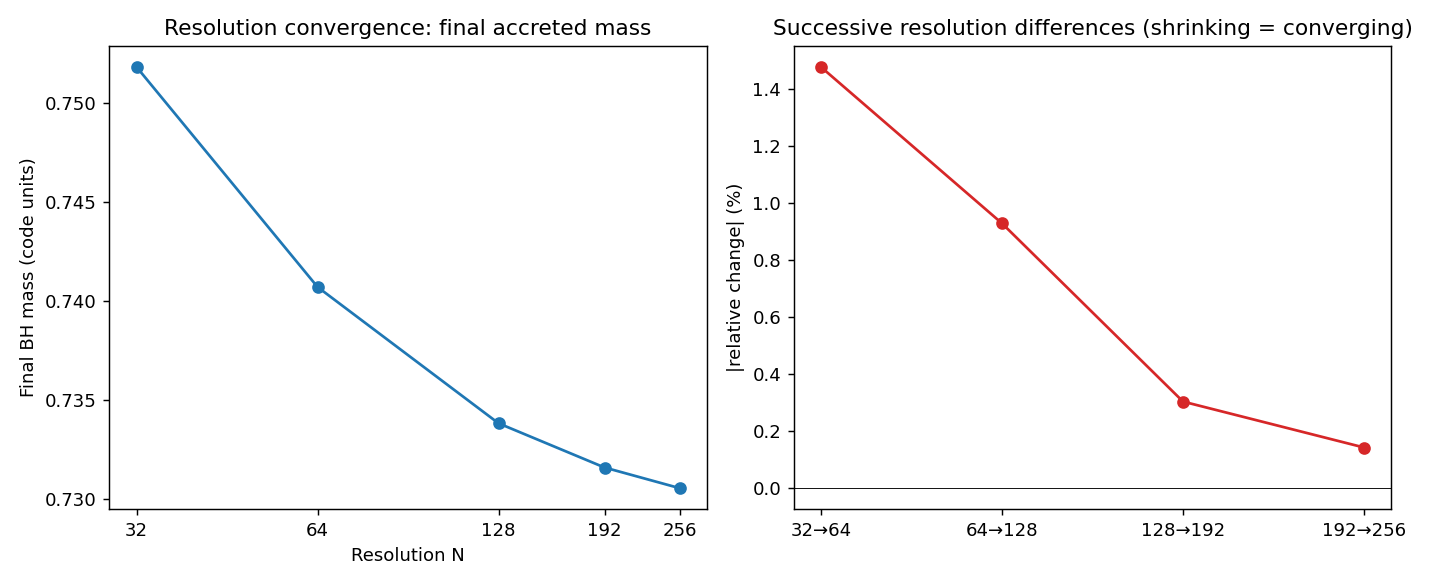
\includegraphics[width=\textwidth]{BHAccretionDemo_convergence.png}
\caption{Final accreted mass vs.\ resolution (left) and successive relative
differences (right), all five resolutions. Successive difference shrinks
$1.48\%\to0.93\%\to0.30\%\to0.14\%$, roughly halving each step — a clean
convergence signature. $192^3$ is within $0.3\%$ of the $256^3$ value;
$128^3$ within $0.9\%$.}
\label{fig:convergence}
\end{figure}

\textbf{Practical reading}: $128^3$--$192^3$ appears to be an adequate
resolution floor for this configuration (sub-1\% and sub-0.5\% of the
$256^3$ answer respectively), pending the same check in the actual campaign
geometries (uniform background / soliton), which may resolve differently.

\OPEN{Wall-time scaling was far steeper than a naive $N^3\times N^2$
(grid cells $\times$ timesteps) estimate suggested, and got worse with
resolution: $64\to128$ was $29\times$ for a $2\times$ bump, $128\to192$ was
$6.5\times$ for $1.5\times$, $192\to256$ was $4.8\times$ for $1.33\times$.
$256^3$ alone took 16 hours on the test machine. Confirmed via repeated
\code{ps}/log checks during the run that this was steady, non-stalled
progress (CPU 165--357\%, regular snapshot cadence) rather than a hang —
reads as thermal throttling under sustained multi-hour load, not a code
bug, but \textbf{unconfirmed on other hardware}. This has real budget
implications for the two campaigns below if they need $\gtrsim192^3$ for
extended durations.}

\section{Immediate next steps}

\begin{enumerate}
  \item Finish \S\ref{sec:convergence}; decide a resolution floor for the
    two campaigns based on it.
  \item Resolve the uniform-background collapse wrinkle (\S1) before or
    alongside starting the dynamical-friction campaign.
  \item Scope and run the stone-skipping campaign: reproduce Zhang et al.'s
    soliton + fixed-mass baseline first (sanity check against their Fig.~1),
    then re-run with accretion on.
  \item \code{MassChange} and \code{Sink.Feedback} both write particle mass
    each step and will clobber each other — needs reconciling before any
    campaign that might touch \code{MassChange}.
\end{enumerate}

\end{document}
